\documentclass[%
 reprint,
%superscriptaddress,
%groupedaddress,
%unsortedaddress,
%runinaddress,
%frontmatterverbose, 
%preprint,
%preprintnumbers,
%nofootinbib,
%nobibnotes,
%bibnotes,
 amsmath,amssymb,
 aps,
%pra,
%prb,
%rmp,
%prstab,
%prstper,
%floatfix,
]{revtex4-2}

\usepackage{graphicx}% Include figure files
\usepackage{dcolumn}% Align table columns on decimal point
\usepackage{bm}% bold math
\usepackage{physics}
%\usepackage{hyperref}% add hypertext capabilities
%\usepackage[mathlines]{lineno}% Enable numbering of text and display math
%\linenumbers\relax % Commence numbering lines

%\usepackage[showframe,%Uncomment any one of the following lines to test 
%%scale=0.7, marginratio={1:1, 2:3}, ignoreall,% default settings
%%text={7in,10in},centering,
%%margin=1.5in,
%%total={6.5in,8.75in}, top=1.2in, left=0.9in, includefoot,
%%height=10in,a5paper,hmargin={3cm,0.8in},
%]{geometry}

\begin{document}

\preprint{APS/123-QED}

\title{Two-Stream Instability using Electrostatic PIC Model}% Force line breaks with \\

\author{Evan Bluhm}
%  \altaffiliation[Also at ]{Physics Department, XYZ University.}%Lines break automatically or can be forced with \\
% \author{Second Author}%
%  \email{Second.Author@institution.edu}
% \affiliation{%
%  Authors' institution and/or address\\
%  This line break forced with \textbackslash\textbackslash
% }%

% \collaboration{MUSO Collaboration}%\noaffiliation

% \author{Charlie Author}
%  \homepage{http://www.Second.institution.edu/~Charlie.Author}
% \affiliation{
%  Second institution and/or address\\
%  This line break forced% with \\
% }%
% \affiliation{
%  Third institution, the second for Charlie Author
% }%
% \author{Delta Author}
% \affiliation{%
%  Authors' institution and/or address\\
%  This line break forced with \textbackslash\textbackslash
% }%

% \collaboration{CLEO Collaboration}%\noaffiliation

\date{April 28, 2021}% It is always \today, today,
             %  but any date may be explicitly specified
\begin{abstract}

The two-stream instability is investigated using a previously implemented 1-dimensional electrostatic particle in cell (PIC) code. A linear analysis of the Vlasov equation is solved to determine unstable modes of two cold, counter-streaming beams of charged particles. The behavior and growth of these unstable modes are demonstrated by the electrostatic PIC code and compared with the predictions from linear theory.

% % \begin{description}
% % \item[Usage]
% % Secondary publications and information retrieval purposes.
% % \item[Structure]
% % You may use the \texttt{description} environment to structure your abstract;
% % use the optional argument of the \verb+\item+ command to give the category of each item. 
% % \end{description}
\end{abstract}

%\keywords{Suggested keywords}%Use showkeys class option if keyword
                              %display desired
\maketitle

%\tableofcontents


\section{Introduction}

The two-stream instability is an excellent example of plasma wave growth that is unstable over time, even in a system very close to equilibrium. A small perturbation in the density in one beam will generate forces leading to a bunching in the opposing beam. The bunching will generate additional forces, amplifying the perturbation exponentially in time.

The behavior of counter-streaming particle beams is an interesting subject for particle-in-cell (PIC) modeling, since even a very simple electrostatic model with a small number of particles can reproduce the solutions predicted by linear Vlasov theory. Here, we use a simple electrostatic PIC model, implemented in Python, to model the time evolution of counter-streaming particle beams.

\section{Linear Analysis}

We consider two 1-dimensional, cold, unmagnetized, counter-streaming electron beams in equilibrium. In the 1-dimensional case, we assume the beams have infinite extent in the $y$ and $z$ direction, and propagate in the $x$ direction. This configuration is homogeneous and static, but as we will see, it is not stable. If we add a small perturbation from the equilibrium state, we would like to know whether such a perturbation grows in time, or decays back to equilibrium. We assume time-harmonic solution modes of our perturbation of the form $e^{i (\omega t - k x)}$, allowing complex values of $\omega$.

The equilibrium particle distribution function for our two-beam system is:
\begin{equation}
f_0 (v) = \frac{1}{2}N \left( \delta(v - v_0) + \delta(v + v_0) \right)
\end{equation}
For a small perturbation $f_1(x, v)$, the distribution function must satisfy the Vlasov equation.
\begin{equation}
\pdv{f}{t} + ( \vec v \cdot \grad)f + \frac{q}{m}(\vec E + \vec v \cross \vec B) \cdot \grad _v f = 0
\end{equation}
Neglecting second-order terms and searching for harmonic plane wave solutions, the linearized Vlasov equation becomes:
\begin{equation}
i (\omega - k v )f_1(v) + \frac{q}{m} \vec E \cdot \grad_v f_0 = 0
\end{equation}
Substituting Poisson's equation and integrating over velocity gives the linearized Vlasov dispersion function $D(k, \omega)$:
\begin{equation}
D(k, \omega) = 1 + \frac{q^2}{m k \epsilon_0} \int_{-\infty} ^{\infty} \frac{\partial f_0 / \partial v}{\omega - k v} \dd v = 0
\end{equation}
For our particular $f_0(v)$, we obtain the dispersion relation:
\begin{equation}
1 - \frac{1}{2} \left( \frac{\omega_p ^2}{(\omega - k v_0)^2} + \frac{\omega_p ^2}{(\omega + k v_0)^2}\right) = 0
\end{equation}
where $\omega_p$ is the usual plasma frequency. There are four independent solutions for the complex $\omega$, as shown in Figure \ref{fig:two-stream-dispersion}:
\begin{equation}
\omega = \pm \sqrt{k^2 v_0 ^2 + \omega_p ^2 \pm \omega_p \sqrt{4 k^2 v_0 ^2 + \omega_p ^2}}
\end{equation}

\begin{figure}
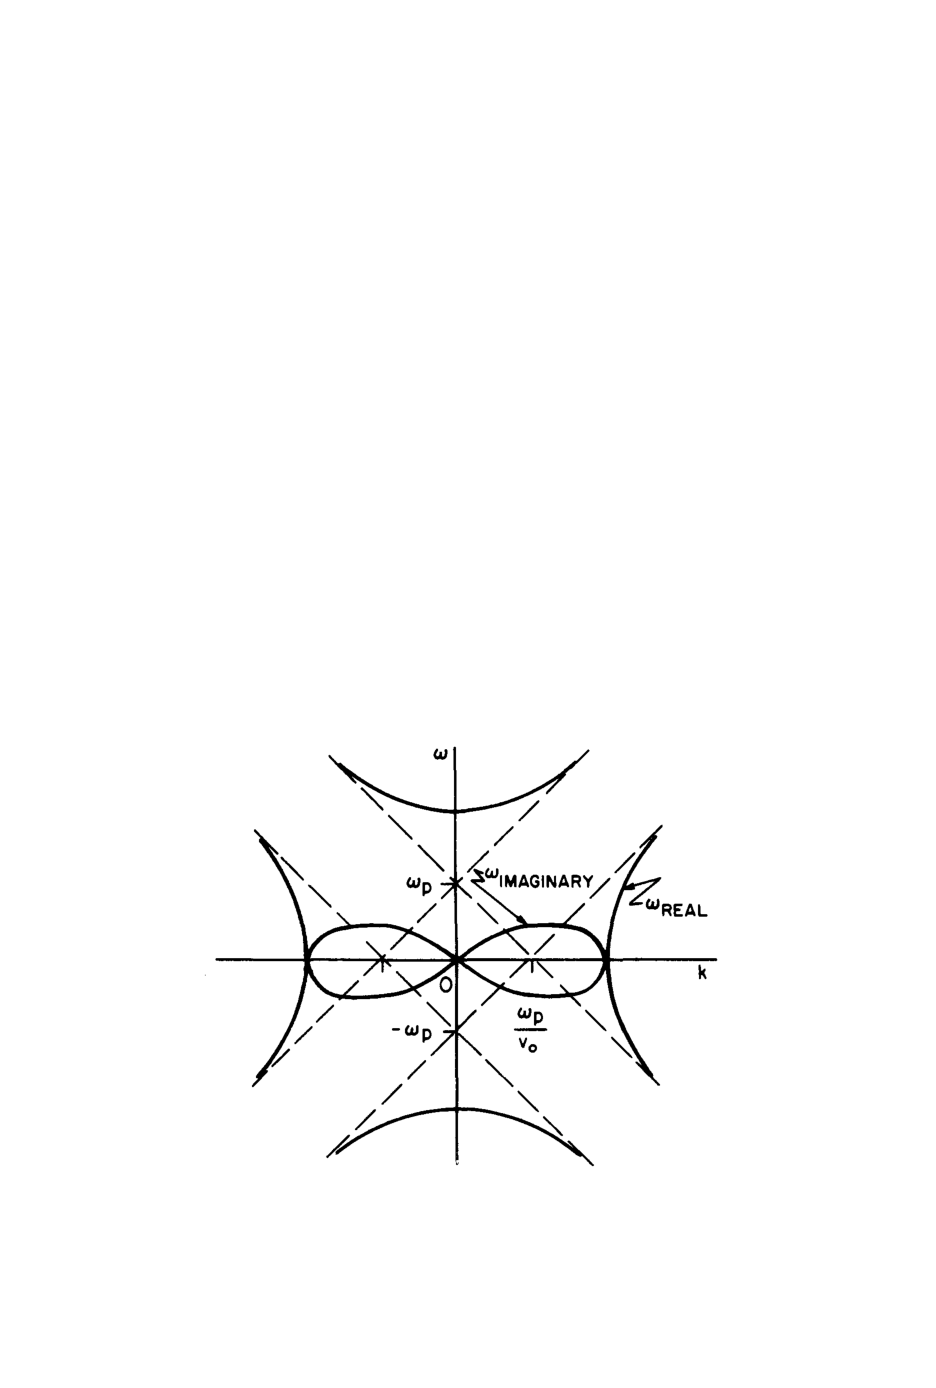
\includegraphics[width=0.9\linewidth]{proj3/birdsall-dispersion-wk.pdf}
\caption{\label{fig:two-stream-dispersion}Dispersion diagram for two equal opposing streams, real $k$, complex $\omega$. The uncoupled space-charge waves are shown dashed. For each value of $k$, there are four values of $\omega$ that correspond to four linearly independent waves. Taken from C. K.  Birdsall, Plasma physics via computer simulation (1991).}
\end{figure}

Interestingly, the system is Hermitian, giving only real-valued eigenvalues. The value $k v_0 / \omega_p$ determines whether each eigenvalue is positive or negative, determining the stability of the eigenmodes. If $0 < k v_0 / \omega_p < \sqrt{2}$, then there are two real solutions and two imaginary solutions for $\omega$. Solutions for which $\omega$ is imaginary will grow exponentially in time, with exponential growth rate $\text{Im}(\omega)$. If $k v_0 / \omega_p > \sqrt{2}$, then all four roots are real and the solution is purely oscillatory.

\section{PIC Model}

We use our previously implemented 1-dimensional electrostatic PIC code to investigate the growth of the two-beam instability modes. The code is initialized with a pair of cold, counter-streaming beams, each containing 512 particles with velocity $\pm v_0$, uniformly spaced over the periodic domain $[- \pi, \pi]$. We then apply a small sinusoidally-varying perturbation of magnitude $\delta=10^{-3}$ to the position of each beam, adding the perturbation to the $+ v_0$ beam and subtracting it from the $- v_0$ beam so that the density bunching is completely out of phase, as shown in Figure \ref{fig:two-stream-initial-density}:
\begin{equation}
{x^0 _i}' = x^0 _i \pm \delta \sin(x^0 _i)
\end{equation}
This perturbation over a single period is expected to excite the longest $k=1$ eigenmode of the linearized Vlasov equation. The other parameters for the simulation are $M = 512$, $\Delta t = 0.01$, and $\omega_p = 1$. The condition for unstable modes to arise is $k v_0 / \omega_p < \sqrt{2}$, so we have set $v_0 = 0.2$ to allow for a range of integer values $k$ in the unstable regime. We integrate forward in time by 20 periods of the plasma frequency and trace out the total kinetic energy, the potential electric field energy, and the particle positions in phase space over time.

\begin{figure}
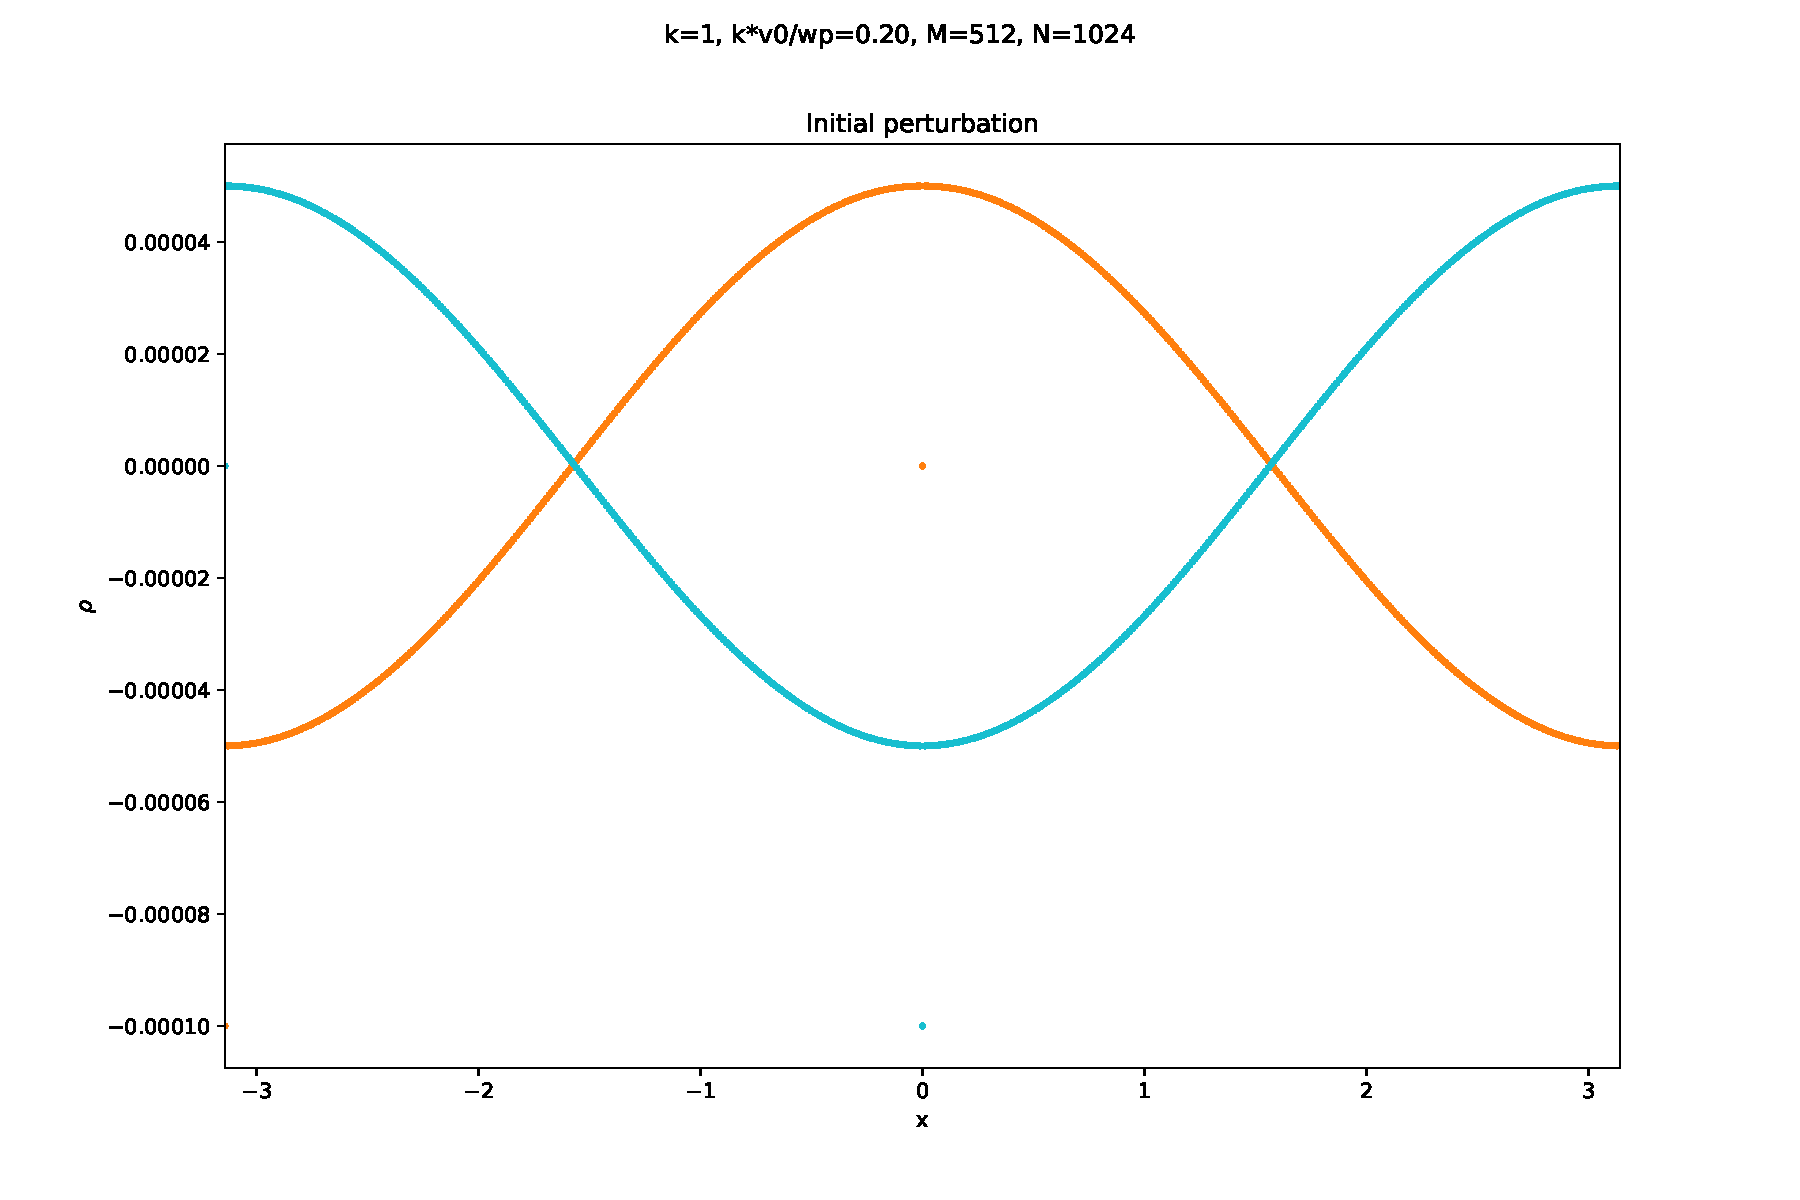
\includegraphics[width=0.9\linewidth]{proj3/two-stream-initial-density.pdf}
\caption{\label{fig:two-stream-initial-density}Initial density perturbation from equilibrium, plotted separately for each beam. The density perturbation is achieved by sinusoidally perturbing the initial positions of the uniformly-spaced particles in each beam. The orange line corresponds with the density perturbation in the forward-propagating beam, and the blue line corresponds with the backwards-propagating beam. The perturbation quantity we are attempting to excite is actually the electric field, related to the density by $\div \vec E = \rho/\epsilon_0$. The density perturbation in each beam is reinforced by bunching in the other, leading to the exponential growth we observe.}
\end{figure}

\section{Results}

\subsection{First Unstable Eigenmode ($k=1$)}

The growth in the unstable eigenmode of the linearized Vlasov equation is readily apparent in the plot of the potential energy stored in the electric field over time, as shown in Figure \ref{fig:two-stream-k=1-energy}. For the model parameters described in the previous section, the imaginary $\omega$ we expect for the $k=1$ mode is:
\begin{equation}
\omega = \sqrt{k^2 v_0 ^2 + \omega_p ^2 - \omega_p \sqrt{4 k^2 v_0 ^2 + \omega_p ^2}} = 0.1924i
\end{equation}
Performing a least squares regression to the linear portion of the growth in the electric field energy, shown in Figure \ref{fig:two-stream-k=1-energy} between $t=23$ and $t=32$, gives an exponential growth constant of $0.381$. Since the potential energy stored in the electric field is proportional to the square of the electric field, $E_{field} \propto \int |\vec E|^2 \dd x$, the growth constant we observe is twice that of the electric field itself. The reduced growth constant $0.381/2 = 1.91$ agrees nicely with the linear theory.

\begin{figure}
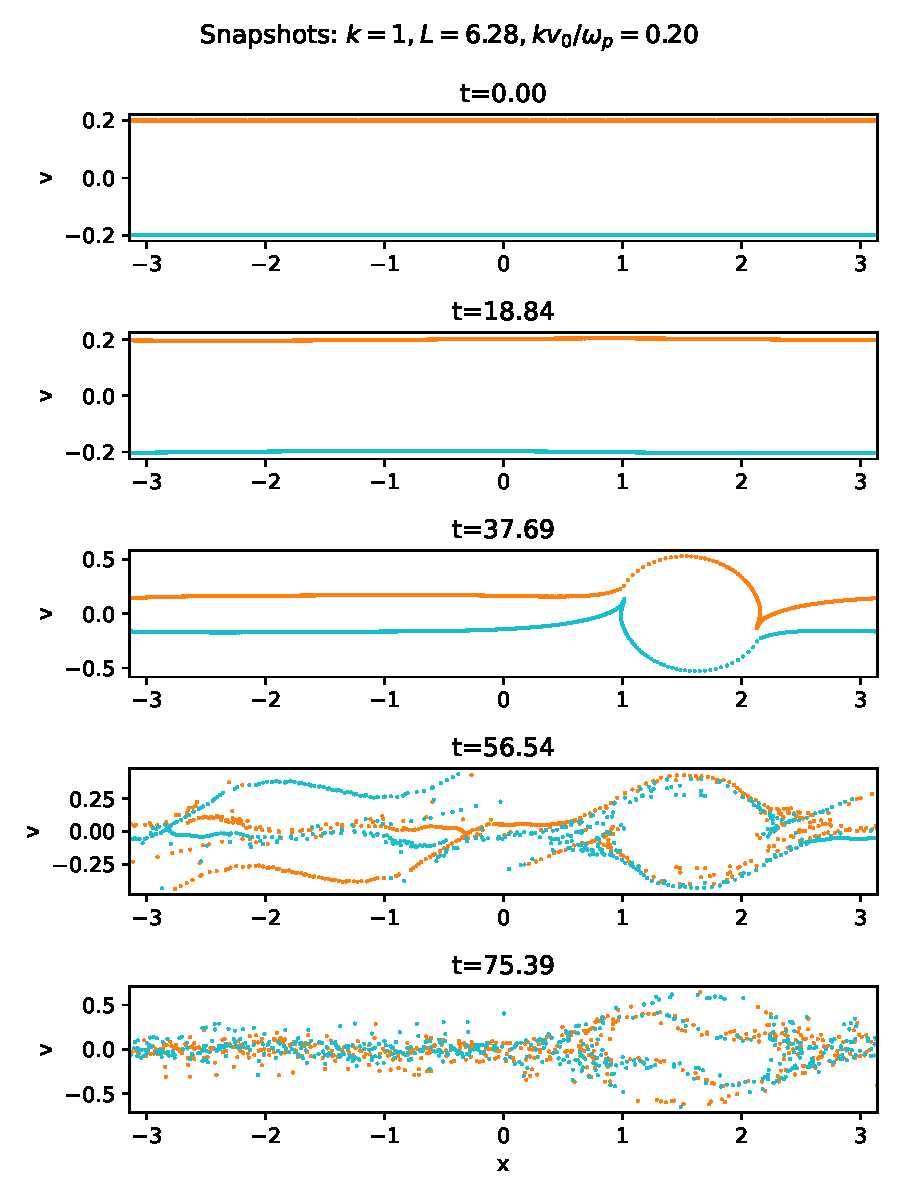
\includegraphics[width=0.9\linewidth]{proj3/two-stream-k=1-snapshots.pdf}
\caption{\label{fig:two-stream-k=1-snapshots}Snapshots of the growth of the $k=1$ two-stream instability over time. Orange particles are initially streaming to the right, and blue particles are initially streaming to the left. $k v_0 / \omega_p = 0.2$, units of time are $1/\omega_p$. The initially small perturbation grows exponentially, appearing as a stationary vortex in phase space. The unstable mode reaches nonlinear saturation after fewer than 10 periods of the plasma frequency.}
\end{figure}

\begin{figure}
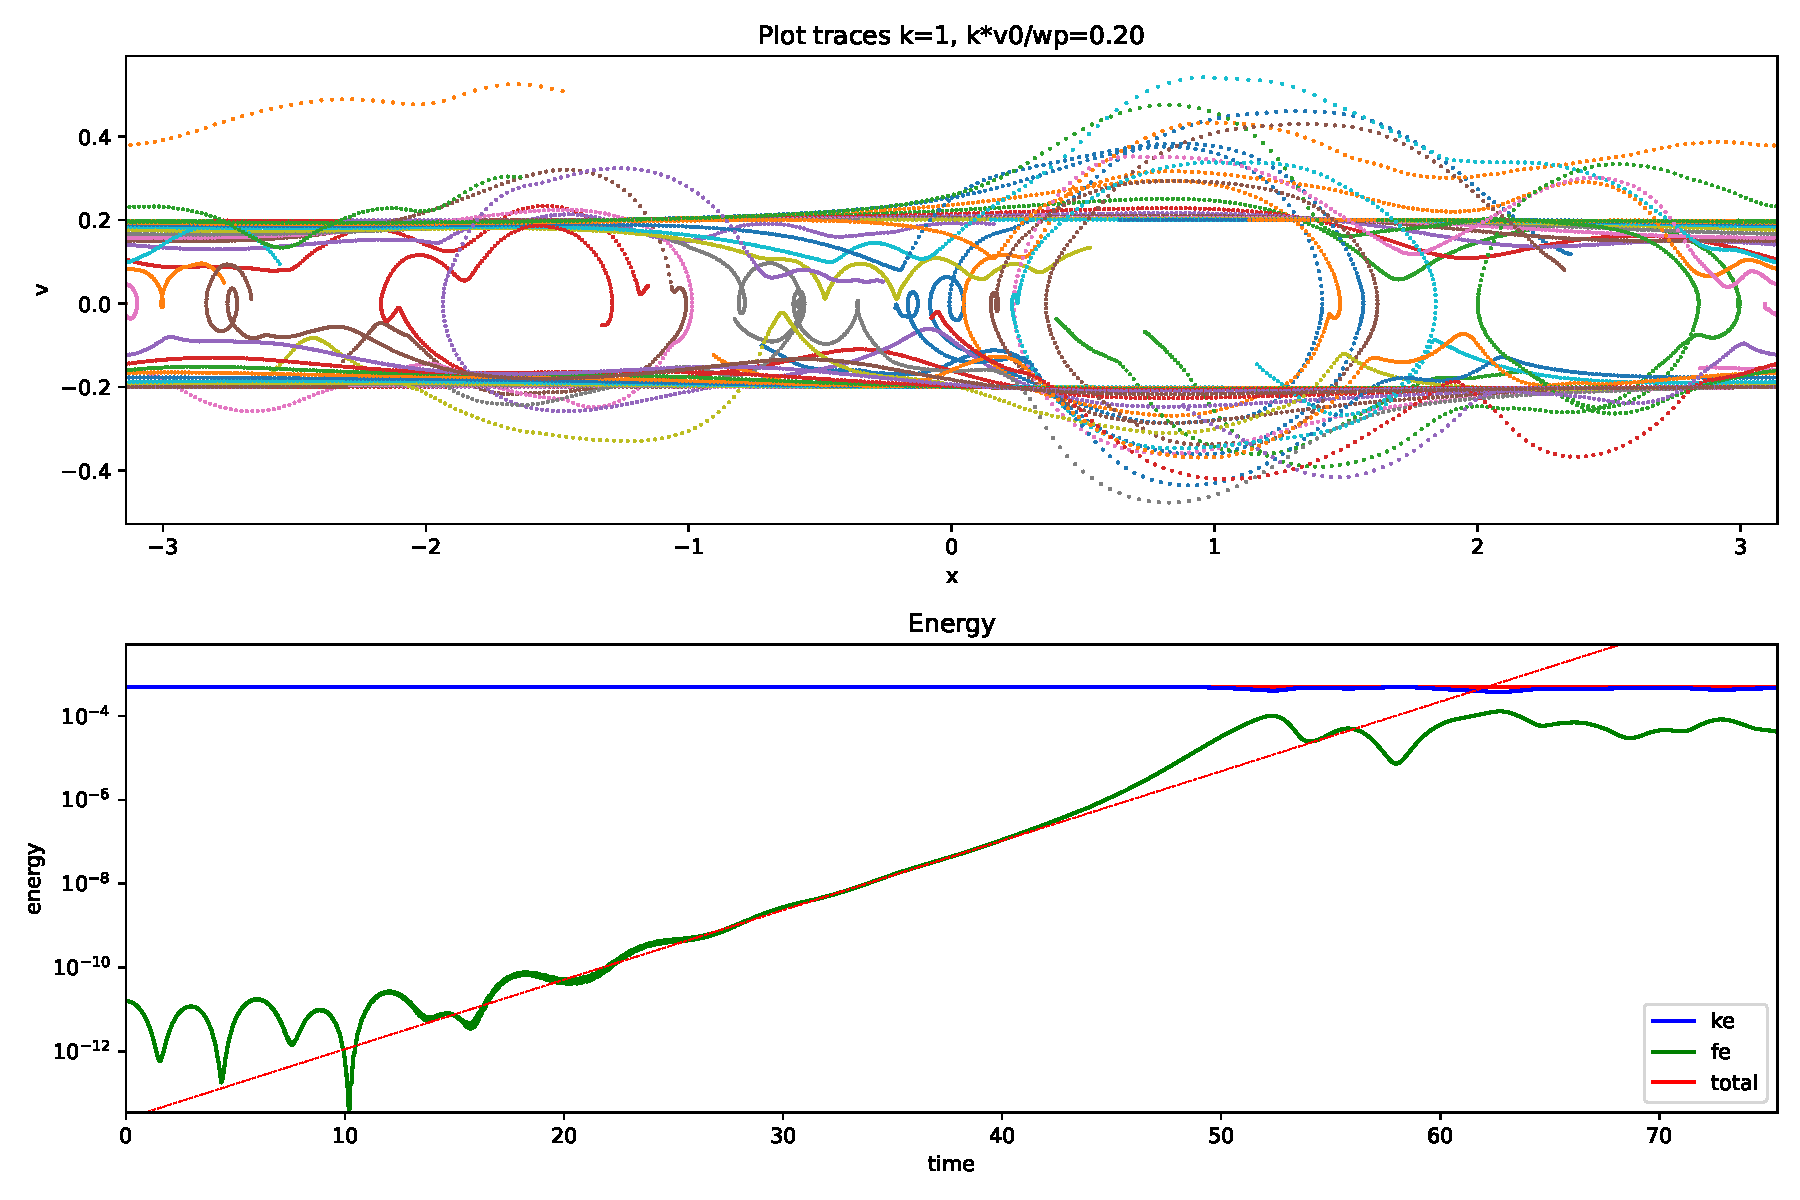
\includegraphics[width=0.9\linewidth]{proj3/two-stream-traces-k=1.pdf}
\caption{\label{fig:two-stream-k=1-energy}Above: Traces of 25 particles in time over the course of the simulation described in Section III. The particle trapping vortex is apparent near $x = 1$. As the unstable modes reach saturation, particles become indefinitely trapped in the vortex by the plasma waves. Below: exponential growth of the total electric field potential energy $\frac{1}{2} \epsilon_0 \int \vec E \cdot \vec E \dd x$. After a brief period of noisy oscillations, the linear growth of the dominant $k=1$ mode becomes apparent. The least squares regression fit to the period of linear growth is shown as a red dashed line, with good agreement with the linear theory.}
\end{figure}

\subsection{Additional Eigenmodes}


\begin{figure}
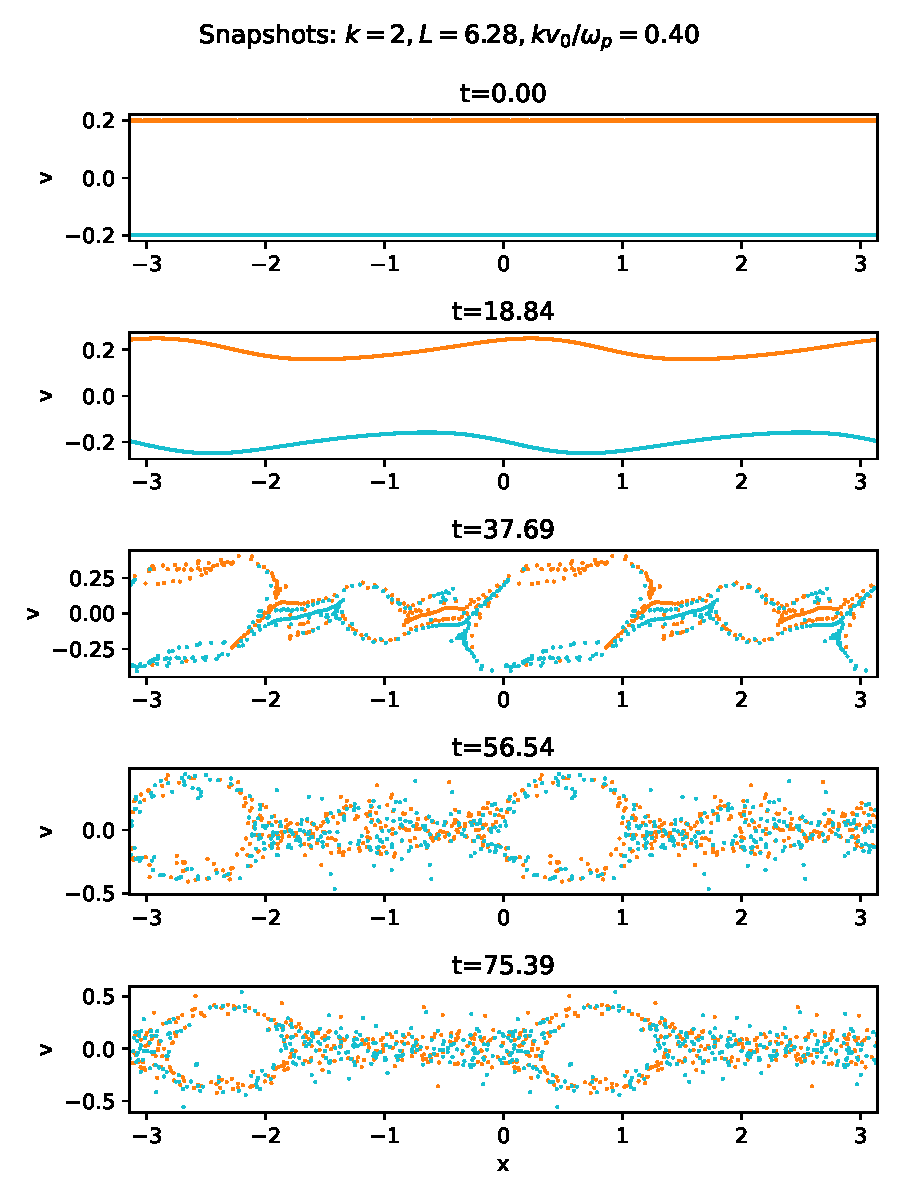
\includegraphics[width=0.9\linewidth]{proj3/two-stream-k=2-snapshots.pdf}
\caption{\label{fig:two-stream-k=2-snapshots}Snapshots of the growth of the $k=2$ two-stream instability over time. $k v_0 / \omega_p = 0.4$, units of time are $1/\omega_p$. In contrast to the $k=1$ initial perturbation, here we see two independent stationary vortexes forming. The $k=2$ instability grows more quickly than the $k=1$, as predicted by the dispersion relation shown in Figure \ref{fig:two-stream-dispersion}.}
\end{figure}

\begin{figure}
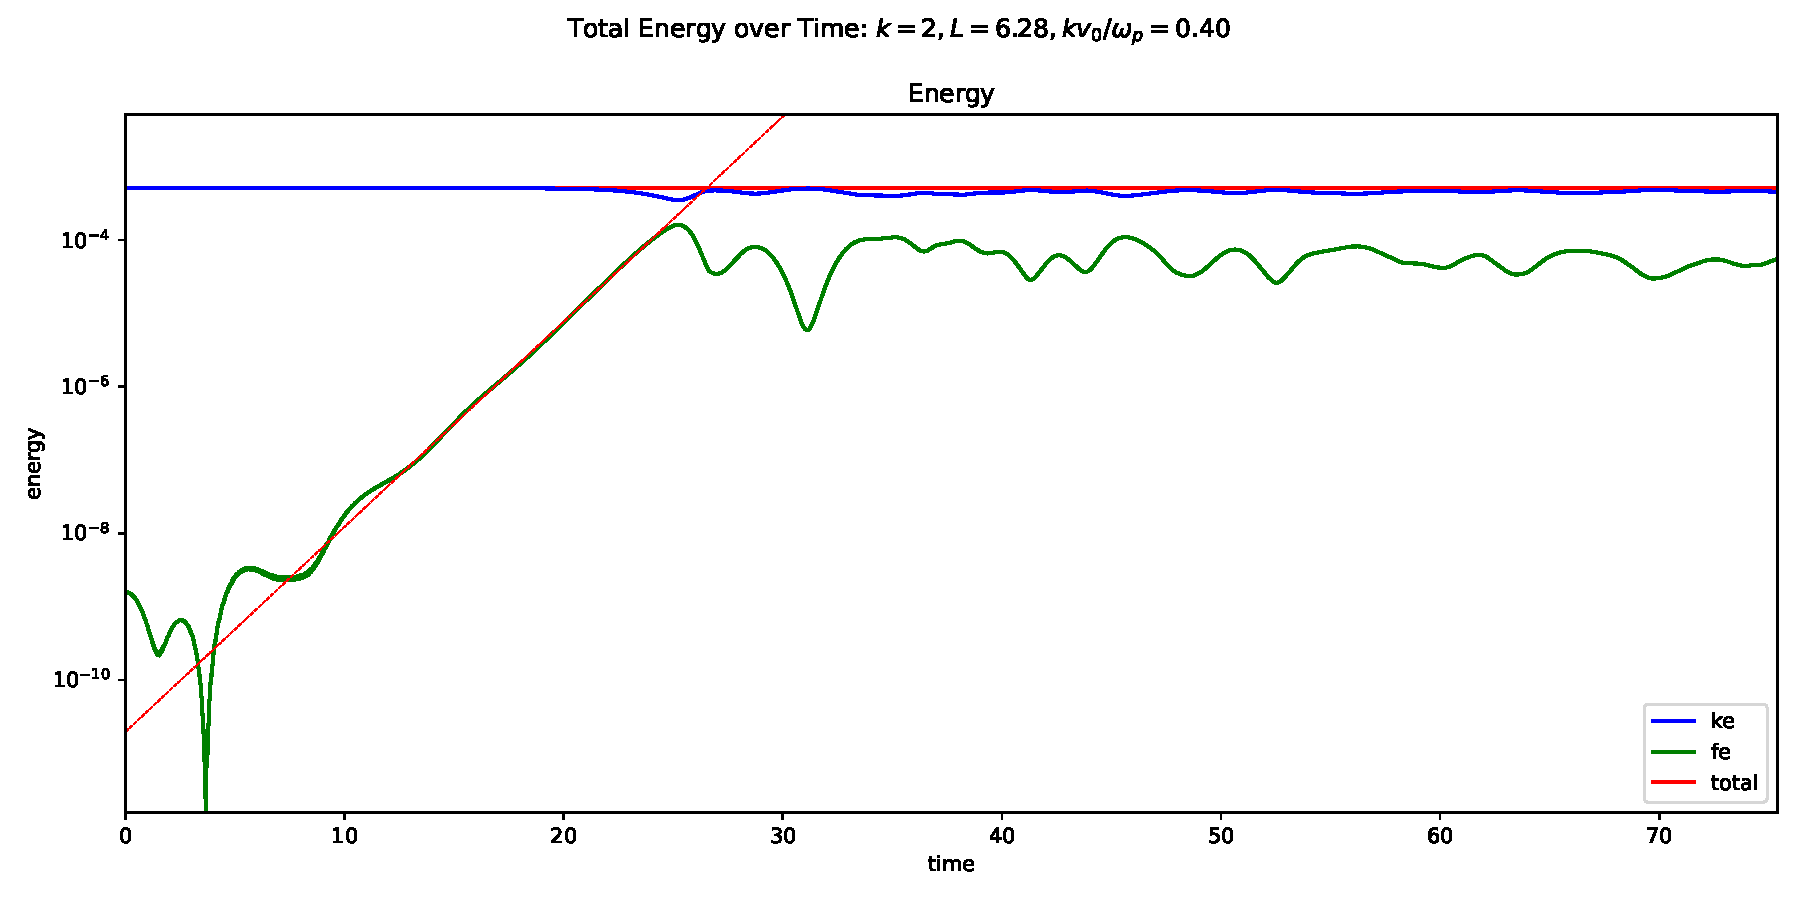
\includegraphics[width=0.9\linewidth]{proj3/energy-k=2-two-stream.pdf}
\caption{\label{fig:two-stream-k=2-energy}Growth of the $k=2$ instability over time, as indicated by the growth of the total potential energy stored in the electric field. The least-squares regression to the linear growth region is shown as a red dashed line, with growth constant $0.643$. The growth constant predicted by the linear theory is $0.695$.}
\end{figure}

\begin{figure}
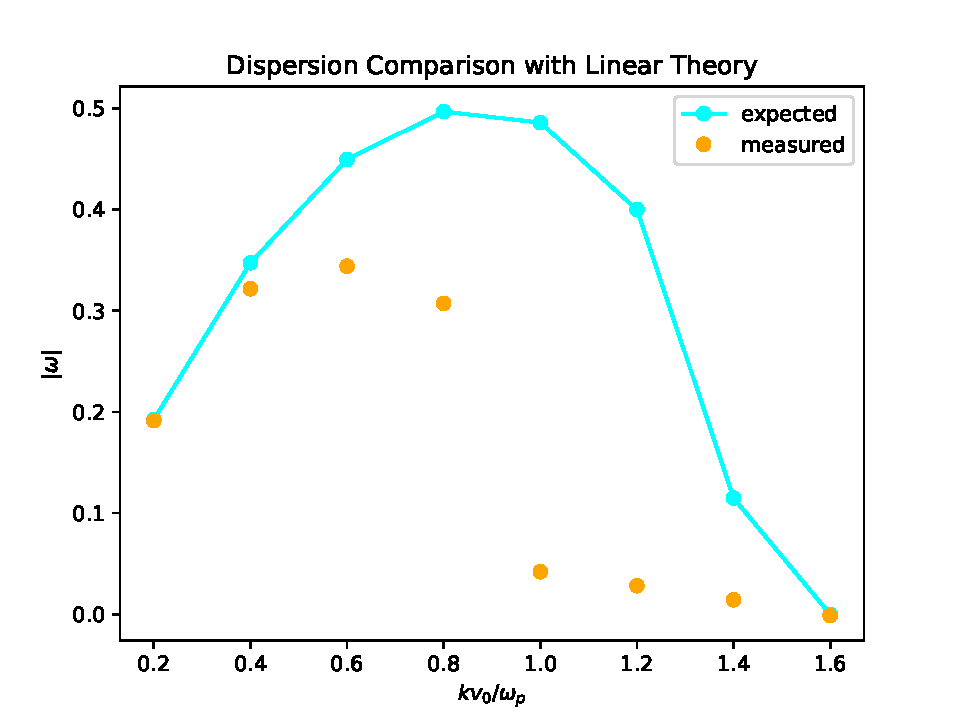
\includegraphics[width=0.9\linewidth]{proj3/dispersion_two_stream.pdf}
\caption{\label{fig:dispersion-measured-comparison}Comparison between the observed growth rate and the growth predicted by linear theory for various values of $k v_0 / \omega_p$. The linear theory predicts the region of instability is $k v_0 / \omega_p < \sqrt{2}$. The growth rate observed in our PIC model agrees at low $k$, but attempting to model higher wavenumber modes is unsuccessful. Snapshots of phase space indicate that when perturbations with higher values of $k$ are applied to the initial conditions, lower-order modes are artificially excited. The low-order excitations may be caused by issues with the stability and accuracy of the PIC model itself.}
\end{figure}


\begin{figure}
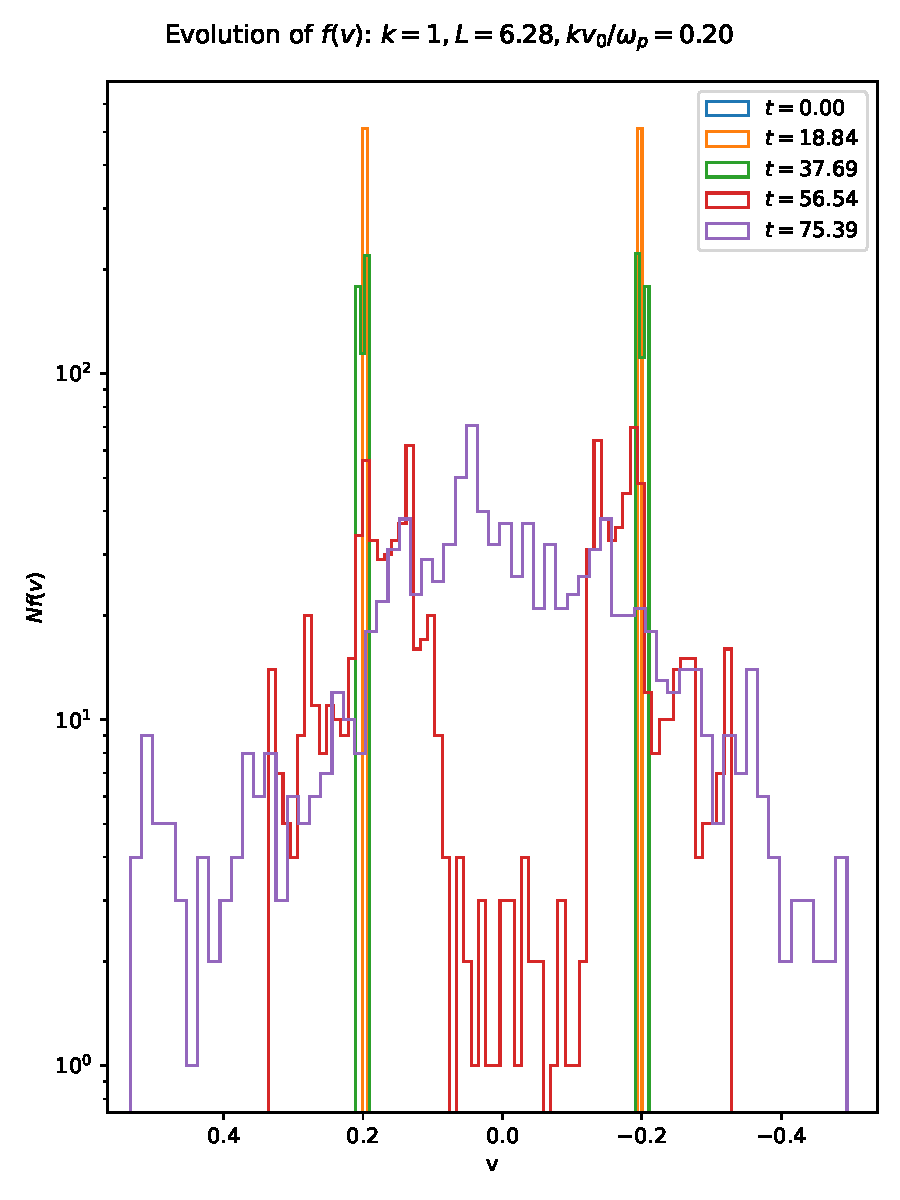
\includegraphics[width=0.8\linewidth]{proj3/fv_hist_1024_particles.pdf}
\caption{\label{fig:fv-evolution-two-stream}Velocity distribution of particles over the course of the simulation described in Section III. Note that the vertical axis is log-scale. The initial distribution is $f_0 (v) = \frac{1}{2}N \left( \delta(v - v_0) + \delta(v + v_0) \right)$, as assumed in the linear analysis in Section II. As unstable modes grow, the velocity distribution of each beam flattens and moves towards $v=0$.}
\end{figure}

By increasing the wavenumber of our initial perturbation, we can observe the growth of higher-wavenumber unstable eigenmodes and compare their growth rate with the linear theory. The growth of the $k=2$ eigenmode is shown in Figure \ref{fig:two-stream-k=2-snapshots}.

Where previously we observed the growth of a single vortex, now there are two independent vortexes which form simultaneously.

Maintaining the same value of $v_0$ and $\omega_p$, the dispersion relation from our linear analysis predicts a growth constant of $\omega = 0.347i$ for $k=2$. The growth of the unstable mode over time is shown in Figure \ref{fig:two-stream-k=2-energy}. The least-squares regression to the region of linear growth (roughly $t=15.5$ to $t=23$) gives $\omega = 0.323$, which is slightly slower than that predicted by the linear theory.

Increasing $k$ further to attempt to excite higher modes begins to diverge from the linear theory for our PIC model. The observed growth rates are compared against those predicted by the linear theory in Figure \ref{fig:dispersion-measured-comparison}. At higher $k$, we see significant divergence from the growth rates predicted by the linear theory. 

\subsection{Relaxation in Velocity Space}


As unstable modes grow and perturb the initially cold beams, the width of each beam in velocity space begins to widen. The time evolution of velocity space is shown in Figure \ref{fig:fv-evolution-two-stream}. At $t=0$, and for several cycles of the plasma frequency afterwards, the two streams remain very sharp peaks in velocity space. As the unstable modes grow, the beams widen. By the end of the simulation run, the velocity space of the two-beam system is much closer to that of a thermal, stationary plasma. Whereas initially the energy of the system resides almost entirely in the bulk velocity of each beam, after fewer than 10 cycles of the plasma frequency the bulk velocity is nearly zero.

This thermalization process has massive ramifications for the prospect of beam-beam fusion. Before the two-stream instability was widely studied, it was hypothesized that beam-beam fusion energy could be easily and efficiently produced by counter streaming ion beams with sufficient bulk velocity to overcome the Coulomb repulsion between ions. Unfortunately, the two-stream instability very rapidly changes the velocity distribution of the system, with the majority of particles losing most of their bulk velocity. The result is that the number of particles with sufficient energy to overcome the Coulomb barrier is many times lower, ruining the efficiency of beam-beam fusion.

\section{Conclusions}

Our simple 1-dimensional electrostatic PIC model was able to demonstrate important features of the two-stream instability, with good agreement with the instability growth predicted by the linearized Vlasov equation. We observe vortex formation and particle trapping characteristic of the two-stream instability. The behavior of our PIC model diverges from the linear theory at higher $k$, indicating possible accuracy and stability issues with the code which will need to be resolved in the future.

The source Python code for the electrostatic PIC model is provided in a .zip archive, along with run instructions and pydoc comments.

% \nocite{*}

% \bibliography{proj3}% Produces the bibliography via BibTeX.

\end{document}
